\documentclass[12pt]{article}
 
\usepackage[margin=1in]{geometry} 
\usepackage{amsmath,amsthm,amssymb,scrextend,mathtools}
\usepackage{fancyhdr}
\pagestyle{fancy}

\usepackage{tikz}
\usepackage[mathscr]{euscript}
\let\euscr\mathscr \let\mathscr\relax% just so we can load this and rsfs
\usepackage[scr]{rsfso}
\usepackage{multicol}
\usepackage{csquotes}
\usepackage[colorlinks=true, pdfstartview=FitV, linkcolor=blue,
citecolor=blue, urlcolor=blue]{hyperref}
\let\ds\displaystyle
\newcommand{\cont}{\subseteq}
\newcommand{\un}{\cup}
\newcommand{\inter}{\cap}
\newcommand{\R}{\mathcal{R}}
\newcommand{\N}{\mathcal{N}}
\newcommand{\E}{\mathbb{E}}
\newcommand{\Var}{\text{Var}}
\newcommand{\Cov}{\text{Cov}}

\usepackage{rotating}
\usepackage{float}
\usepackage{graphicx}
\usepackage{placeins}

% Tighter, more stable float placement (reduces large whitespace gaps)
\setlength{\textfloatsep}{6pt plus 1pt minus 1pt}
\setlength{\floatsep}{6pt plus 1pt minus 1pt}
\setlength{\intextsep}{4pt plus 1pt minus 1pt}
\renewcommand{\topfraction}{0.9}
\renewcommand{\bottomfraction}{0.8}
\renewcommand{\textfraction}{0.07}
\renewcommand{\floatpagefraction}{0.8}

\begin{document}
 

\lhead{PhD CorpFin -- Maxted}
\chead{Logan Casey}
\rhead{\today}
 
\section*{Campbell Presidential Lecture}
\subsection*{Figure 1}
The wealth distribution looks broadly similar; the tails are a bit different but could be due to differences in the sample/weights (including decisions made in my code), not changes in reality. Note that the x-axis variable is different for each y variable; the ordering of households total assets is not the same as the ordering by financial assets or net worth.
\begin{figure}[H]
    \centering
    \includegraphics[width=0.85\textwidth]{wealth_dist.png}
\end{figure}

\begin{figure}[H]
    \centering
    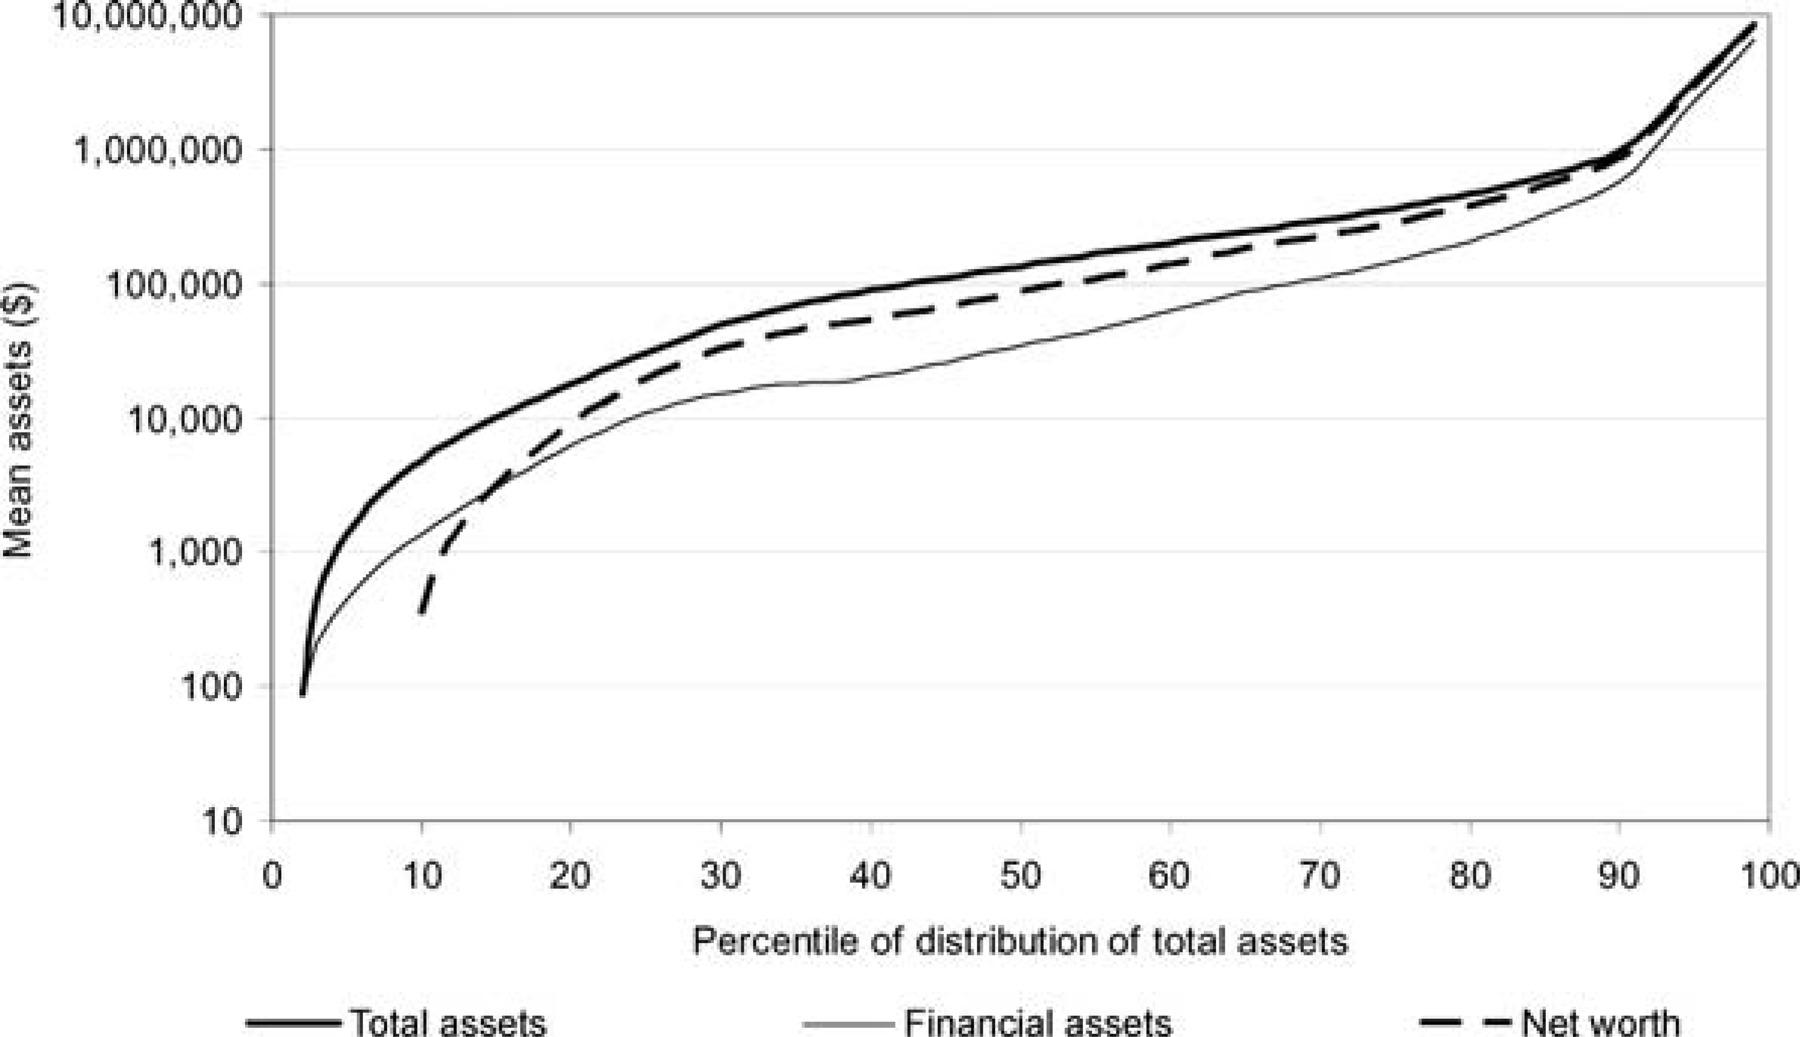
\includegraphics[width=0.75\textwidth]{campbell1.jpg}
\end{figure}


\clearpage
\subsection*{Figure 2}
Other than the missing zeroes at the bottom of the distribution, this also looks quite similar. I smoothed the plot data (lpoly in Stata) for clarity; Campbell does not mention smoothing, but it seems likely given the noise when using 100 bins. Also note that bonds are not shown on Campbell's figure but are mentioned in the text; this is the variable that required the most discretion to construct. Public equity is perhaps in more household wealth portfolios; real estate in fewer.
\begin{figure}[H]
    \centering
    \includegraphics[width=0.85\textwidth]{participation_by_asset_percentile.png}
\end{figure}

\begin{figure}[H]
    \centering
    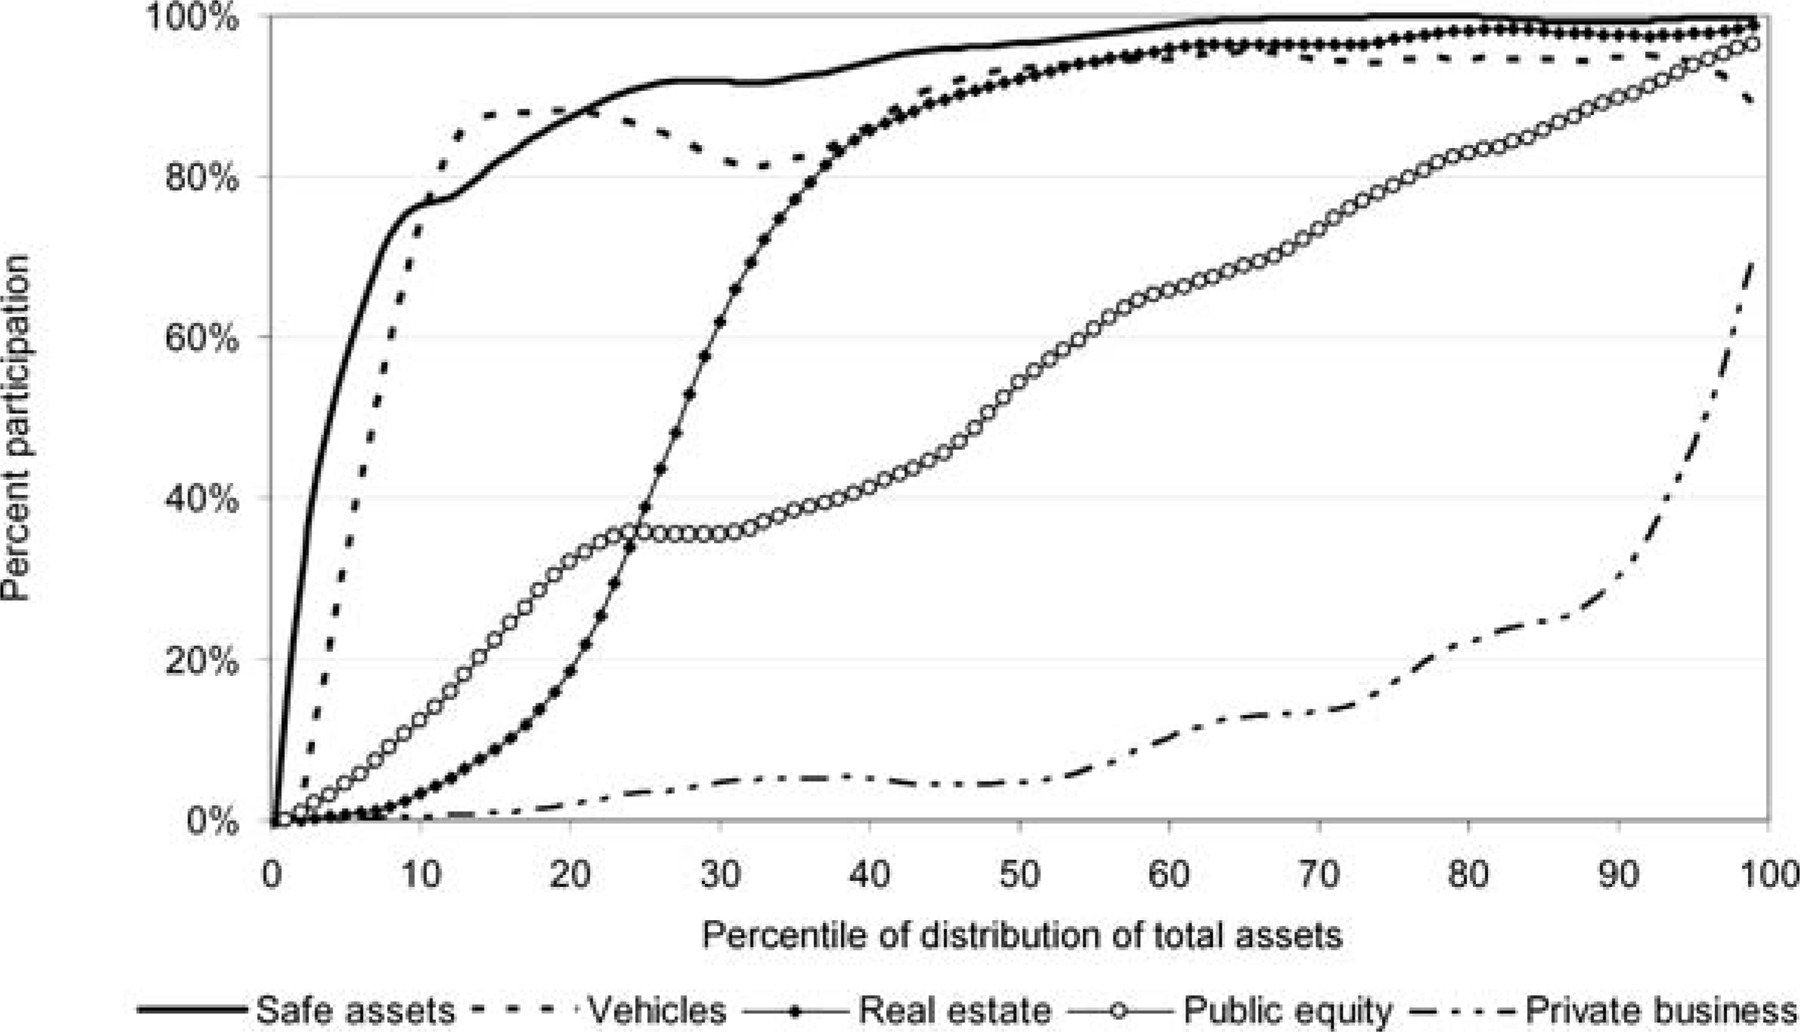
\includegraphics[width=0.75\textwidth]{campbell2.jpg}
\end{figure}

\clearpage
\subsection*{Figure 3}
This figure is also smoothed. The plot shows the share of the plot-level total; otherwise the asset categories do not add to 100\%. I am not sure why this is; it does not seem to be that some households are missing data entirely. With that caveat the facts in each graph are similar. The importance of business ownership and public equity at the top end is more muted in the 2022 figure -- this is an artifact of smoothing for business ownership but not for public equity.
\begin{figure}[H]
    \centering
    \includegraphics[width=0.85\textwidth]{portfolio_shares_by_asset_percentile.png}
\end{figure}

\begin{figure}[H]
    \centering
    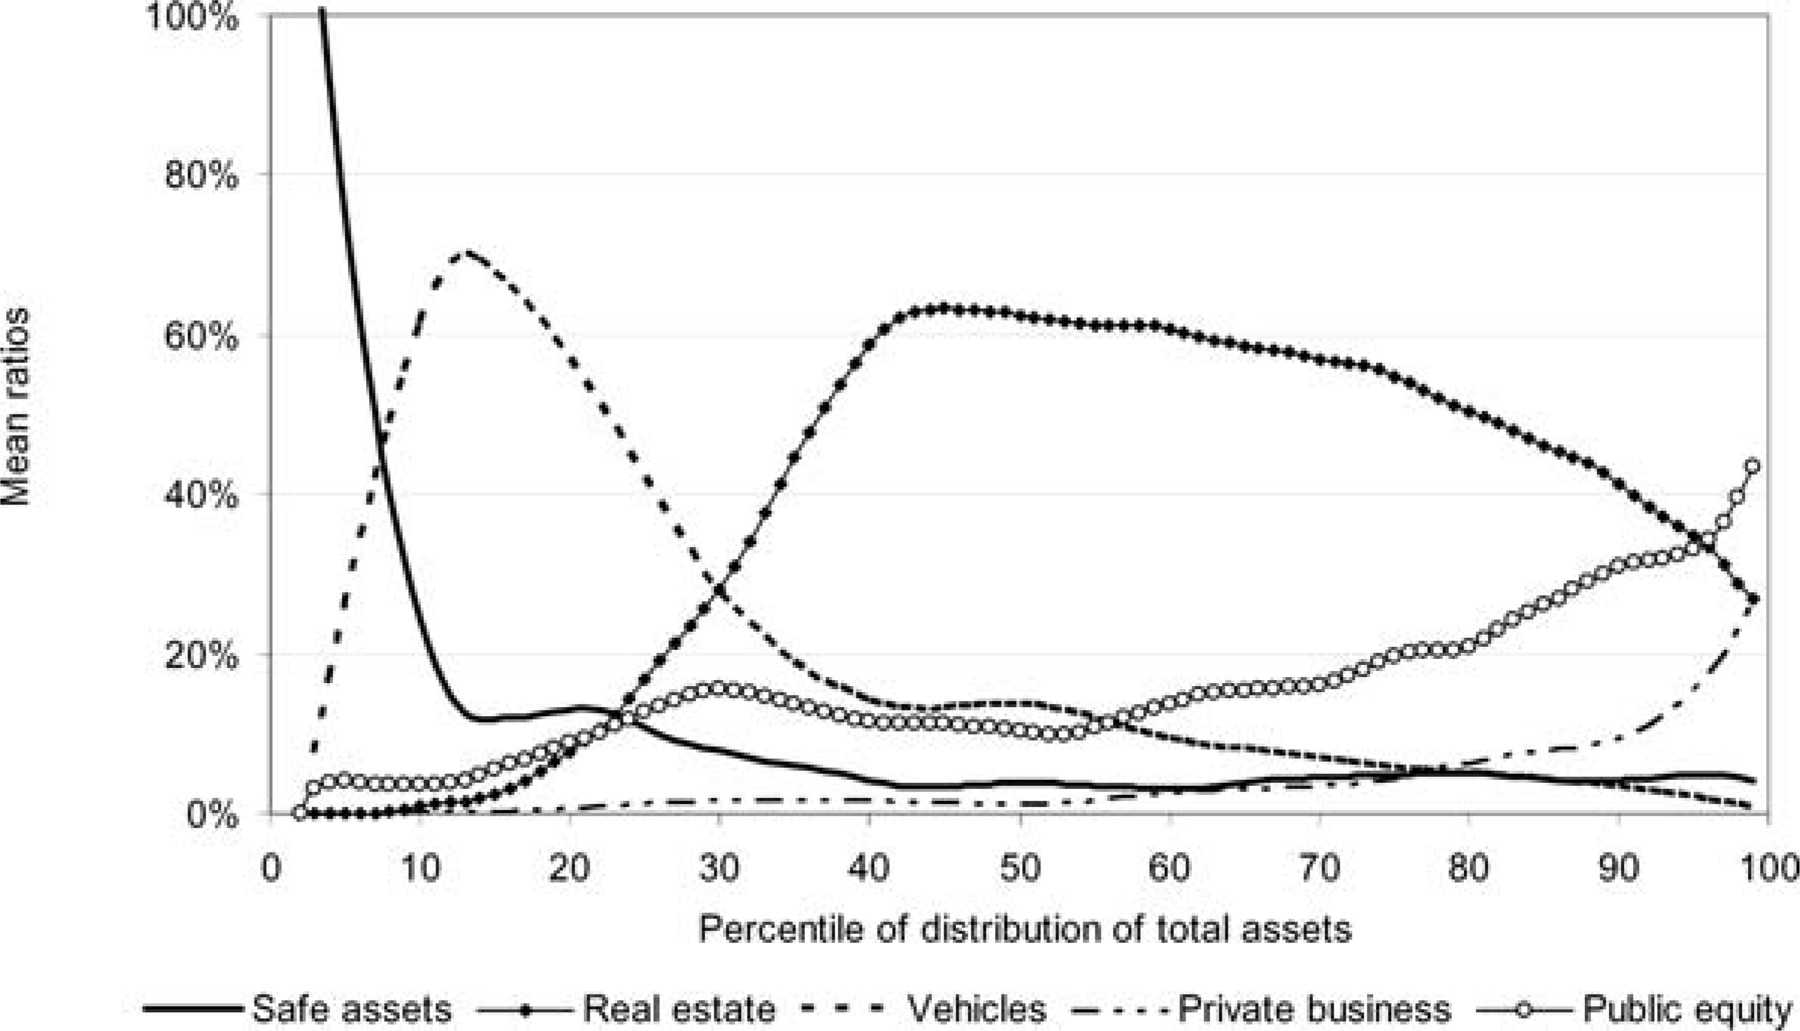
\includegraphics[width=0.75\textwidth]{campbell3.jpg}
\end{figure}

\clearpage
\section*{Hand-to-mouth households}
Using Kaplan \& Violante's definition (\$\$ in bank accounts < 0.5 months' income), 37.1\% of households are hand-to-mouth. If we include money-market and call accounts, the share is 33.6\%. If we also include CDs and prepaid cards, it is 31.3\%. If we include public equity, it is 21.7\% (note this is not just directly held stocks). Intuitively, it makes sense to me that \enquote{hand-to-mouth} households may have high net worth because they own homes and vehicles. Owning stocks is a bit trickier. I am curious to read more about the behavioral interpretation of high MPCs. I would also be curious about asymmetry in sign of MPCs -- I could imagine households with financial resources but little cash use those resources to smooth negative income shocks.

\section*{Credit-card debt}
If we drop zeroes, 56\% of households have revolving credit-card debt, and 62\% of those with credit cards (Reference in Peter's paper -- 52\%). The average (as well as median) interest rate is 17\% (16\%).

\end{document}
